\documentclass[crop=false]{standalone}
\begin{document}
	\section{Methodology}
	\subsection{System Overview}
	系統架構如圖一所示,由RGBD攝影機拍攝具有深度影像資訊後,將RGB影像與深度影像輸入進YOLO物件偵測模型。交由深度學習模型負責執行物件偵測,再由模型偵測到的物件位置轉換座標系後給DWA動態調整路徑。此外,加入最短路徑演算法,提升 DWA在評選路徑時的速度。此最短路徑能使得無人機以最少時間情況下抵達指定的地點,並且能夠避開障礙物。
	
	\begin{figure*}[thbp!]
		\centering
		\fbox{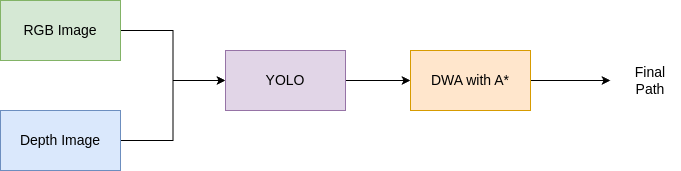
\includegraphics[width=\textwidth]{furtherwork_workflow}}
		\caption{The system architecture}
		\label{fig:system}
	\end{figure*}
	\subsection{General Kinematics Model}
	本文實驗使用無人機,並且假設在固定高度且固定速度下進行,這使得局部路徑規劃問題可以簡化成在2維空間上的路徑規劃問題。DWA 將機器人的位置控制問題轉成速度控制問題,並利用速度控制預測機器人運動軌跡。為此,需要先分析機器人運動模型\cite{fox},令$x(t), y(t)$為在$t$時間下,機器人的世界座標系下的位姿,且令機器人的方向為$\theta(t)$,則機器人運動可被表達為$<x, y, \theta>$,令機器人的平移速度為$v$,轉向加速度為$\omega(t)$,則一般來說可以表達如下:
	
	\begin{equation}
		x(t_n)=x(t_0)+ \int_{t_0}^{t_n}v(t) \cdot cos(\theta)dt
	\end{equation}
	\begin{equation}
		y(t_n)=y(t_0)+ \int_{t_0}^{t_n}v(t) \cdot sin(\theta)dt
	\end{equation}
	\begin{equation}
		\theta(t)=\theta(t_0)+\int_{t_0}^{t_n}\omega(t)dt
	\end{equation}
	
	
	\subsection{Objective Function}
	因為有多種不同的平移速度和角速度,所以需要從不同的平移速度和角速度的組合形成的路徑中挑選一條最佳的路徑,挑選的方式則是透過以下目標函數進行評比:
	\begin{equation}
		G(v, \omega)=\sigma(\alpha Heading(v, \omega) + \beta Obstacle(v, \omega) + \gamma Velocity(v, \omega))
	\end{equation}
	\begin{itemize}
		\item Heading function - 此函數用來使得機器人保持朝向終點方向前進,$\theta$ 愈小代表機器人與終點的方向角愈小。
		\item Obstacle avoidance function - 本文中障礙物為靜態障礙物,且每次隨機生成。在已知障礙座標下,可計算機器人與障礙物之間的距離$dist$,$dist$透過歐基里德公式計算後可得到。如果機器人碰到障礙物的距離大於機器人半徑,則可被視為沒有發生碰撞。
		\item Velocity function - 機器人平移前進的速度
	\end{itemize}
	$\sigma$ 函數則是對三個函數進行標準化
	\begin{equation}
		normalHead(i)=\frac{head(i)}{\sum_{i=1}^{n}{head(i)}}
	\end{equation}
	\begin{equation}
		normalDist(i)=\frac{dist(i)}{\sum_{i=1}^{n}{dist(i)}}
	\end{equation}
	\begin{equation}
		normalVelocity(i)=\frac{velocity(i)}{\sum_{i=1}^{n}{velocity(i)}}
	\end{equation}
	其中n為所有採樣的軌跡,i為現在等待評比的當前軌跡
\end{document}